\begin{problem}{C}{Conan-kun, Please Stop Shooting Kogoro}{1 second}

\noindent
Kogoro is investigating a city consisting of $N$ districts connected by $M$ two-way roads. The $i$-th road connects districts $u_i$ and $v_i$ and has length $w_i$. It is possible to travel between every pair of districts.

\noindent
Kogoro carefully wrote down the endpoints and length of every road on a board. Unfortunately, just as Conan fired his tranquilizer needle at him, Kogoro collapsed onto the board and erased the lengths of the last $K$ roads.

\noindent
Fortunately, Kogoro still remembers the $K$ erased values: $A_1,A_2,\ldots,A_K$. However, he no longer remembers which value belonged to which road.

\noindent
For a path $P$ from district $1$ to district $N$:

\begin{itemize}
   \item The \textbf{best-case length} of $P$ is the minimum possible length of $P$ over all assignments of the erased weights.
   \item The \textbf{worst-case length} of $P$ is the maximum possible length of $P$ over all assignments of the erased weights.
   \item The \textbf{expected length} of $P$ is the expected length of $P$ when the assignment of the erased weights is chosen uniformly at random.
\end{itemize}

\noindent
Among all possible paths from district $1$ to district $N$, find the minimum best-case length, the minimum worst-case length, and the minimum expected length. The paths that minimize these three values are not necessarily the same.

\InputFile

\noindent
The first line contains a single integer $T$ --- the number of test cases.

\noindent
Each test case consists of the following lines.

\noindent
The first line contains three integers $N$, $M$, and $K$ $(2 \le N \le 10^4,\ N-1 \le M \le 10^4,\ 1 \le K \le \min(M,100))$ --- the number of districts, the number of roads, and the number of roads whose lengths were erased, respectively.

\noindent
Each of the next $M-K$ lines contains three integers $u_i$, $v_i$, and $w_i$ $(1 \le u_i,v_i \le N,\ u_i \ne v_i,\ 1 \le w_i \le 10^4)$ --- the endpoints and the length of the $i$-th road.

\noindent
Each of the next $K$ lines contains two integers $u_i$ and $v_i$ $(1 \le u_i,v_i \le N,\ u_i \ne v_i)$ --- the endpoints of the $i$-th road whose length was erased.

\noindent
The next line contains $K$ integers $A_1,A_2,\ldots,A_K$ $(1 \le A_i \le 10^4)$ --- the erased road lengths.

\noindent
It is guaranteed that all unordered pairs $(u_i,v_i)$ are distinct, the graph is connected, and the sum of $M$ over all test cases does not exceed $10^4$.

\OutputFile

\noindent
For each test case, print one line containing three integers $B$, $W$, and $E$ --- the minimum best-case length, the minimum worst-case length, and the minimum expected length, respectively. The answer for each test case should be printed on a separate line.

\noindent
For the expected length, if its value can be represented as an irreducible fraction $\frac{p}{q}$, print $ E = p \cdot q^{-1} \bmod 998244353$ where $q^{-1}$ denotes the multiplicative inverse of $q$ modulo $998244353$.

\Examples

\begin{example}
\exmp{1}{1
4 5 2
1 2 1
1 3 2
3 4 1
2 4
1 4
4 1
}{1 3 499122179
}
\end{example}

\Note

\begin{center}
  \def \htmlPixelsInCm {45}
  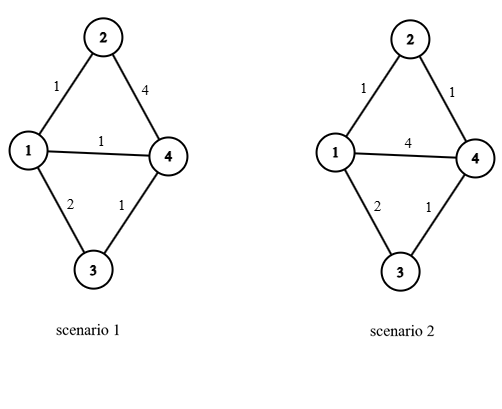
\includegraphics[width=0.55\textwidth]{./assets/C.png} \\
  \small{Fig. 1: Illustration of all possible scenarios in the sample case.}
\end{center}

\noindent
Fig. 1 illustrates all possible scenarios for the sample case.

\begin{itemize}
    \item Path $1 \to 4$ minimizes the best-case length, which is $1$.
    \item Path $1 \to 3 \to 4$ minimizes the worst-case length, which is $3$. The worst-case length of path $1 \to 4$ is $4$, as shown in Scenario 2.
    \item Path $1 \to 4$ minimizes the expected length, which is $(4 + 1) / 2$. Therefore, the expected length is printed as $5 \cdot 2^{-1} \bmod 998244353$.
\end{itemize}

\pagebreak

\end{problem}